\begin{prob}
    In the following, let
    \begin{align*}
        V &= \{0,1,2,3,4,5,6,7\},\\
        E &= \{
        (0,1), 
        (1,5), 
        (5,2), 
        (0,5), 
        (7,3),
        (6,7) 
    \}.
    \end{align*}

    For this problem, you do not need to show your work.

    \begin{subprobset}
        \begin{subprob}
            Draw the \emph{undirected} graph $G = (V,E)$. Remember that when
            writing the edges of an undirected graph, we often abuse
            notation and write $(u,v)$ when we really mean $\{u,v\}$; we
            have done so here.

            \begin{soln}

                \begin{center}
                \begin{tikzpicture}[
                    every node/.style={draw, thick, circle, minimum width=2em}
                    ]
                    \node (0) at (-3,-1) {$0$};
                    \node (1) at (-1,1) {$1$};
                    \node (2) at (-0.5,-2.5) {$2$};
                    \node (6) at (6,-1.5) {$6$};
                    \node (3) at (5,0.5) {$3$};
                    \node (5) at (-1,-1) {$5$};
                    \node (4) at (2,-1) {$4$};
                    \node (7) at (8, 0.5) {$7$};

                    \foreach \i/\j in {0/1,1/5,5/2,0/5,7/3,6/7}{
                        \draw (\i) edge (\j);
                    }
                \end{tikzpicture}
                \end{center}

            \end{soln}
        \end{subprob}

        \begin{subprob}
            Draw the graph $G = (V,E)$, assuming that $G$ is directed.

            \begin{soln}

                \begin{center}
                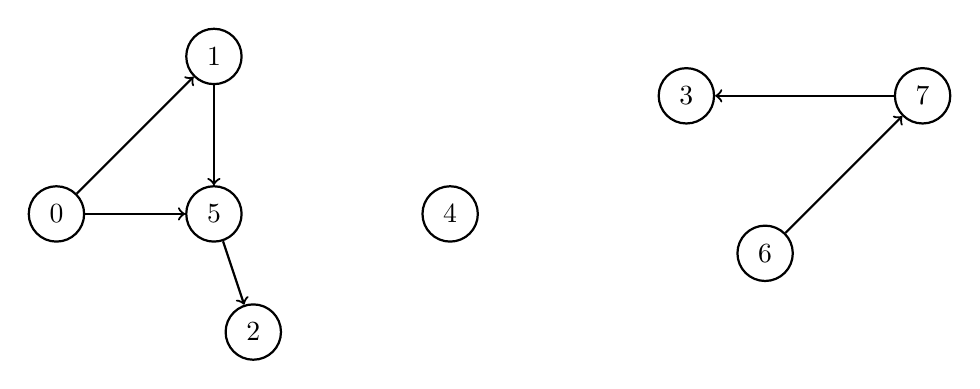
\begin{tikzpicture}[
                    every node/.style={draw, thick, circle, minimum width=2em}
                    ]

                    \node (0) at (-3,-1) {$0$};
                    \node (1) at (-1,1) {$1$};
                    \node (2) at (-0.5,-2.5) {$2$};
                    \node (6) at (6,-1.5) {$6$};
                    \node (3) at (5,0.5) {$3$};
                    \node (5) at (-1,-1) {$5$};
                    \node (4) at (2,-1) {$4$};
                    \node (7) at (8, 0.5) {$7$};

                    \foreach \i/\j in {0/1,1/5,5/2,0/5,7/3,6/7}{
                        \draw (\i) edge[->, thick] (\j);
                    }

                \end{tikzpicture}
                \end{center}

            \end{soln}
        \end{subprob}

        \begin{subprob}
            Write down the connected components of $G$, assuming that $G$ is undirected.

            \begin{soln}
                From the above drawing we see that the connected components
                are:
                \[
                    \{0, 1, 2, 5\}, \{3, 6, 7\}, \{4\}
                \]
            \end{soln}
            
        \end{subprob}

        \begin{subprob}
            Write the adjacency matrix representation of $G$, assuming that G is undirected.

            \begin{soln}

                \[
                \begin{pmatrix}
                    0 & 1 & 0 & 0 & 0 & 1 & 0 & 0\\
                    1 & 0 & 0 & 0 & 0 & 1 & 0 & 0\\
                    0 & 0 & 0 & 0 & 0 & 1 & 0 & 0\\
                    0 & 0 & 0 & 0 & 0 & 0 & 0 & 1\\
                    0 & 0 & 0 & 0 & 0 & 0 & 0 & 0\\
                    1 & 1 & 1 & 0 & 0 & 0 & 0 & 0\\
                    0 & 0 & 0 & 0 & 0 & 0 & 0 & 1\\
                    0 & 0 & 0 & 1 & 0 & 0 & 1 & 0\\
                \end{pmatrix}
                \]

            \end{soln}
        \end{subprob}

        \begin{subprob}
            Write the adjacency matrix representation of $G$, assuming that G is directed.

            \begin{soln}

                \[
                \begin{pmatrix}
                    0 & 1 & 0 & 0 & 0 & 1 & 0 & 0\\
                    0 & 0 & 0 & 0 & 0 & 1 & 0 & 0\\
                    0 & 0 & 0 & 0 & 0 & 0 & 0 & 0\\
                    0 & 0 & 0 & 0 & 0 & 0 & 0 & 0\\
                    0 & 0 & 0 & 0 & 0 & 0 & 0 & 0\\
                    0 & 0 & 1 & 0 & 0 & 0 & 0 & 0\\
                    0 & 0 & 0 & 0 & 0 & 0 & 0 & 1\\
                    0 & 0 & 0 & 1 & 0 & 0 & 0 & 0\\
                \end{pmatrix}
                \]

            \end{soln}
            
        \end{subprob}

    \end{subprobset}
\end{prob}
